\chapter{Конструкторская часть}
В данном разделе будет рассмотрены схемы исследуемого алгоритма.

\section{Схемы алгоритмов}

На рисунке \ref{fig:alg1} представлена схема однопоточного алгоритма блочной сортировки.

На рисунке \ref{fig:alg2} представлена схема распараллеленного алгоритма блочной сортировки.

На рисунке \ref{fig:alg3} представлена схема алгоритма сортировки вставками, используемой для сортировки каждого блока.

На рисунке \ref{fig:alg4} представлена схема пареллельного выполнения цикла.

\begin{figure}[h!]
	\centering
	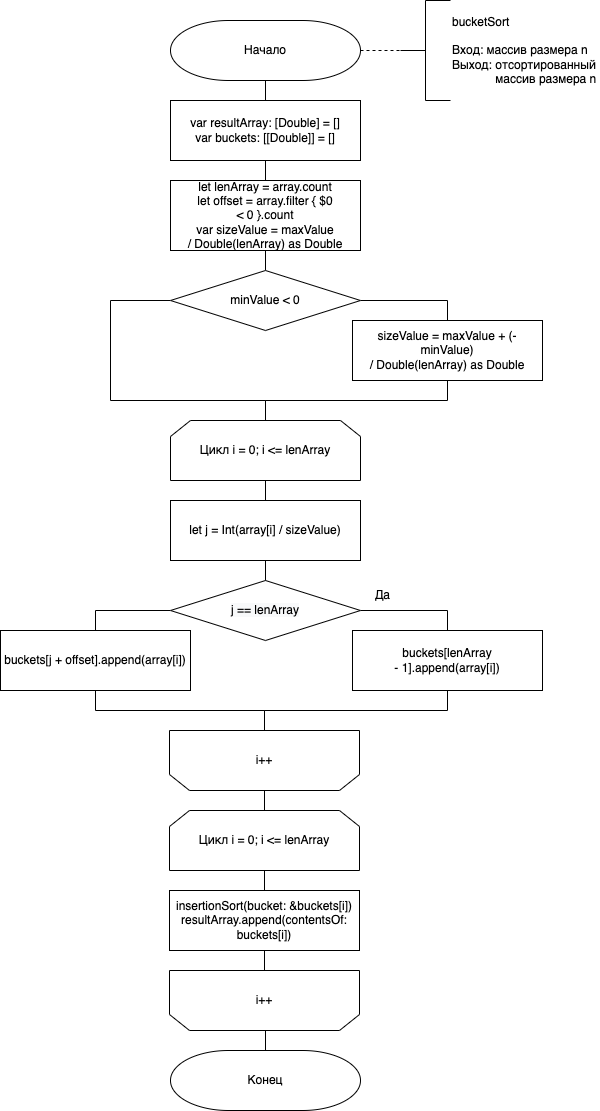
\includegraphics[width=0.8\linewidth]{img/Bucket.png}
	\caption{Схема алгоритма блочной сортировки}
	\label{fig:alg1}
\end{figure}

\begin{figure}[h!]
	\centering
	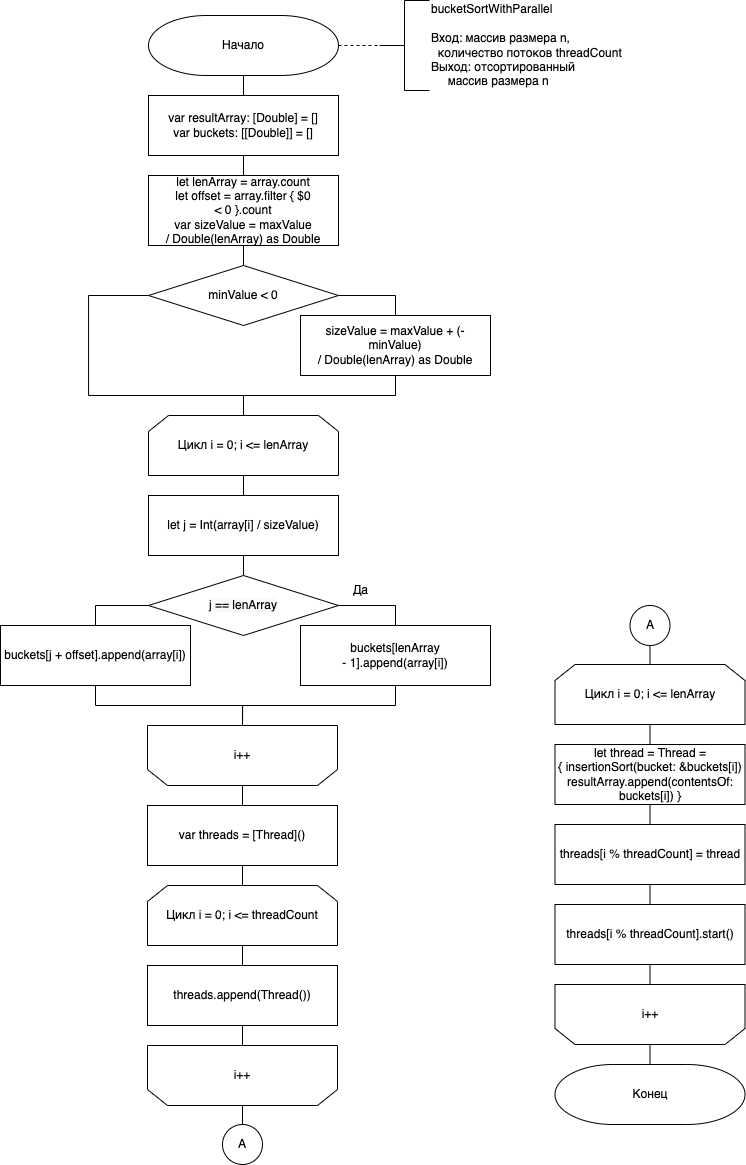
\includegraphics[width=0.95\linewidth]{img/BucketParallel.png}
	\caption{Схема алгоритма блочной сортировки параллельно}
	\label{fig:alg2}
\end{figure}

\begin{figure}[h!]
	\centering
	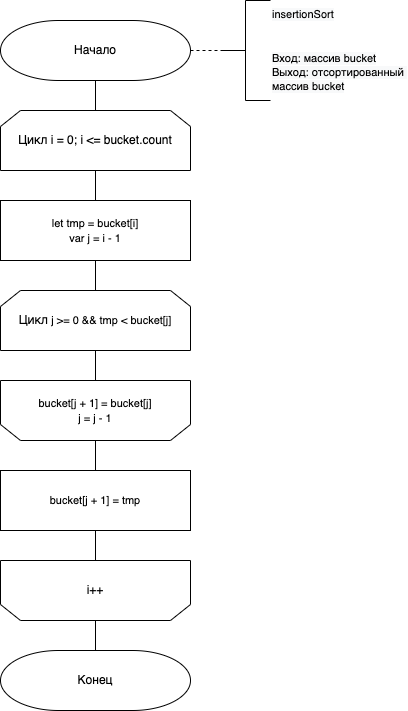
\includegraphics[width=0.6\linewidth]{img/Insertion.png}
	\caption{Схема алгоритма блочной сортировки}
	\label{fig:alg3}
\end{figure}


\begin{figure}[h!]
	\centering
	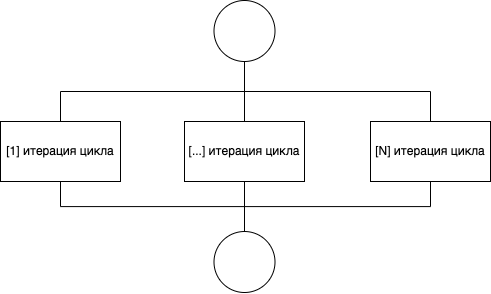
\includegraphics[width=0.6\linewidth]{img/Threads.png}
	\caption{Схема с параллельным выполнением цикла}
	\label{fig:alg4}
\end{figure}


\section{Вывод}
На основе теоретических данных, полученных из аналитического раздела, была построена схема стандартного алгоритма блочной сортировки, а также, после разделения алгоритма на этапы, была предложена схема параллельного выполнения этапов.
